\documentclass[dvisvgm]{minimal}
\usepackage{tikz}

% Set font from website
\usepackage[T1]{fontenc}
\usepackage[default]{sourcesanspro}

% Set colors from website
\usepackage{xcolor}
\definecolor{qe-gray}{RGB}{68,68,68}
\definecolor{qe-blue}{RGB}{0, 114, 188}

\begin{document}
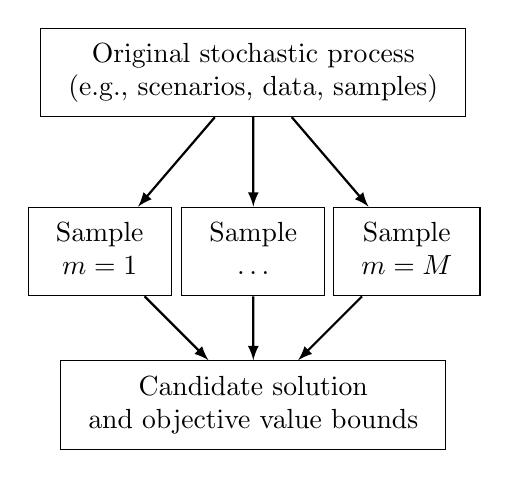
\begin{tikzpicture}[scale=1.3]
%		    \draw[help lines] (0,0) grid (4,8);
			\node[draw, inner sep=4pt] (original) at (2,7) {\begin{tabular}{cc} Original stochastic process \\ (e.g., scenarios, data, samples) \end{tabular}};
			\node[draw, inner sep=4pt] (sample1) at (0.5,5.25) {\begin{tabular}{cc} Sample \\ $m=1$ \end{tabular}};
			\node[draw, inner sep=4pt] (sample2) at (2,5.25) {\begin{tabular}{cc} Sample \\ $\dots$ \end{tabular}};
			\node[draw, inner sep=4pt] (sample3) at (3.5,5.25) {\begin{tabular}{cc} Sample \\ $m=M$ \end{tabular}};
			\node[draw, inner sep=4pt] (SAA) at (2,3.75) { \begin{tabular}{cc} Candidate solution \\ and objective value bounds \end{tabular}};
			\draw[-latex, thick] (original) -- (sample1);
			\draw[-latex, thick] (original) -- (sample2);
			\draw[-latex, thick] (original) -- (sample3);
			\draw[-latex, thick] (sample1) -- (SAA);
			\draw[-latex, thick] (sample2) -- (SAA);
			\draw[-latex, thick] (sample3) -- (SAA);
		\end{tikzpicture}
\end{document}